\documentclass[border=0.1cm]{standalone}
\usepackage{tikz}
\usetikzlibrary{
  decorations.text
  }
%
\begin{document}
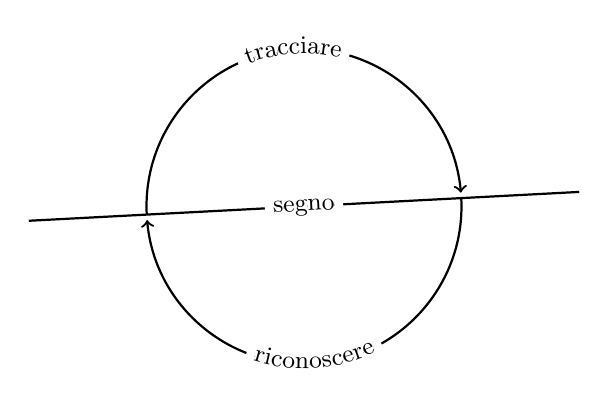
\begin{tikzpicture}
  \tikzstyle{every node}=[font=\small]
  \begin{scope}[rotate=3]
    \draw[thick, postaction={
      decorate,
      decoration={
        raise=-1.7pt,
        text effects along path,
        text align=center,
        text={~segno~},
        text effects/.cd,
          character count=\i,
          character total=\n,
          characters={text along path, fill=white}}}
          ] (-0.5,0) -- (6.5,0);
      %node[fill=white, midway, sloped, inner ysep=0pt]{\tiny creazione};
    \draw[thick, ->, postaction={
      decorate,
      decoration={
        raise=-1.7pt,
        text effects along path,
        text align=center,
        text={~tracciare~},
        text effects/.cd,
          character count=\i,
          character total=\n,
          characters={text along path, fill=white}}}
        ] (1,0) arc (180:2:2cm);
      %node[fill=white, midway, sloped, inner ysep=0pt]{\tiny ricerca};
    \draw[thick, ->, postaction={
      decorate,
      decoration={
        raise=-1.7pt,
        text effects along path,
        reverse path,
        text align=center,
        text={~riconoscere~},
        text effects/.cd,
          character count=\i,
          character total=\n,
          characters={text along path, fill=white}}}
          ] (5,0) arc (0:-178:2cm);
      %node[fill=white, midway, sloped, inner ysep=0pt]{\tiny invenzione};
  \end{scope}
  %
 \end{tikzpicture}

\end{document}
